\section{\texorpdfstring{Program Pole - indexové adresování}{Program Pole - indexove adresovani}}

% =====================================================================================================================
	\begin{frame}
    \frametitle{Zadání}

		\begin{enumerate}
			\item Program spustí světelný efekt na LED přípravku,
			\vspace{3mm}
			\item LED budou rozsvěceny dle pevného zadání v paměti,
			\vspace{3mm}
			\item pro časování programu bude použita již napsaná funkce \textbf{wait}.
		\end{enumerate}
		
	\end{frame}
	
% =====================================================================================================================
	\begin{frame}
    \frametitle{Výstupní port s LED u přípravku}
		
		\begin{center}
			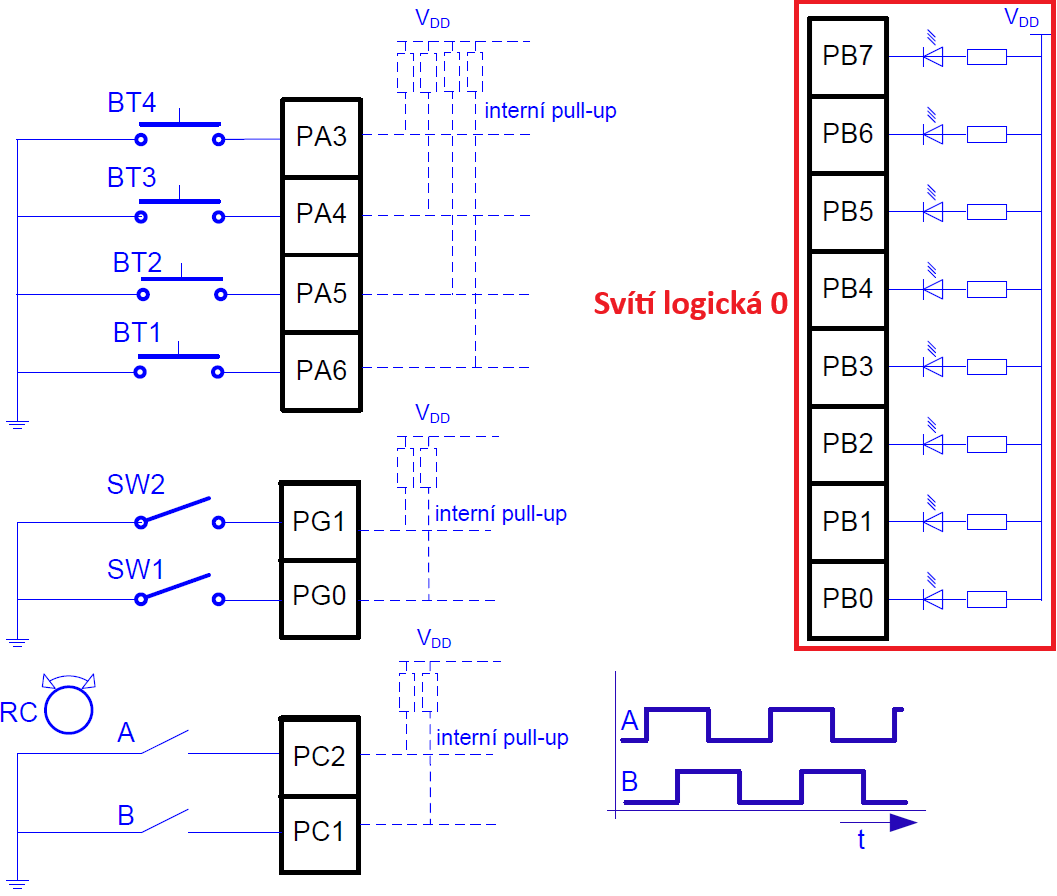
\includegraphics[width=0.65\textwidth]{fig/ports_out.png}
		\end{center}
		
	\end{frame}
	
% =====================================================================================================================
	\begin{frame}
    \frametitle{Nastavení pinu procesoru}
		
		\begin{center}
			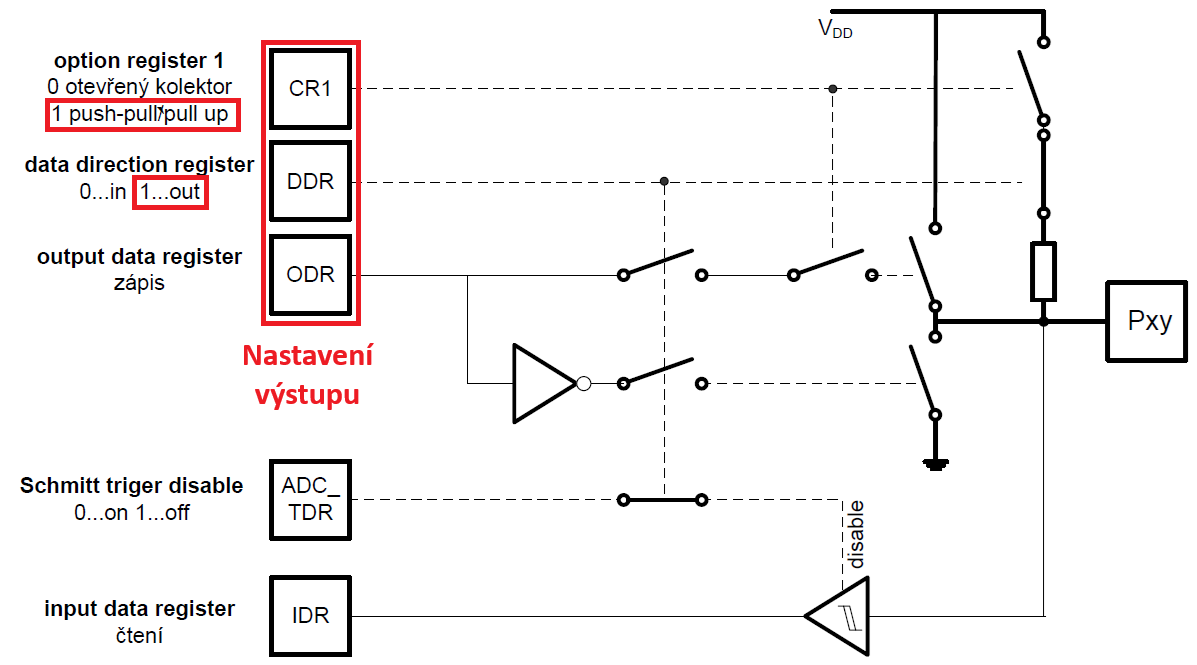
\includegraphics[width=0.90\textwidth]{fig/pin_settings_out.png}
		\end{center}
		
	\end{frame}
	
% =====================================================================================================================
	\begin{frame}
    \frametitle{Program - definiční konstanty}
		
		\begin{center}
			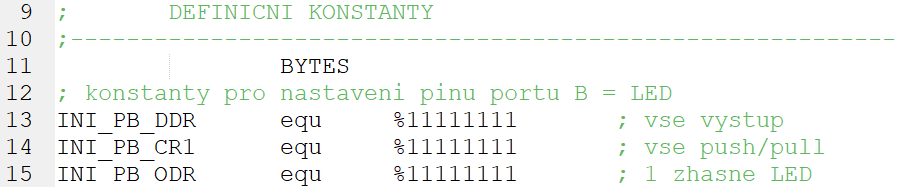
\includegraphics[width=0.80\textwidth]{fig/prg_pole_konst.png}
		\end{center}
		
		\begin{itemize}
			\item pojmenované hodnoty = konstanty,
			\item překladač nahradí název konstanty její hodnotou,
			\item pojmenování usnadňuje případný přepis konstanty, pokud se nachází na více místech v programu.
		\end{itemize}
		
	\end{frame}
	
% =====================================================================================================================
	\begin{frame}
    \frametitle{Program - hlavní smyčka}
		
		\begin{center}
			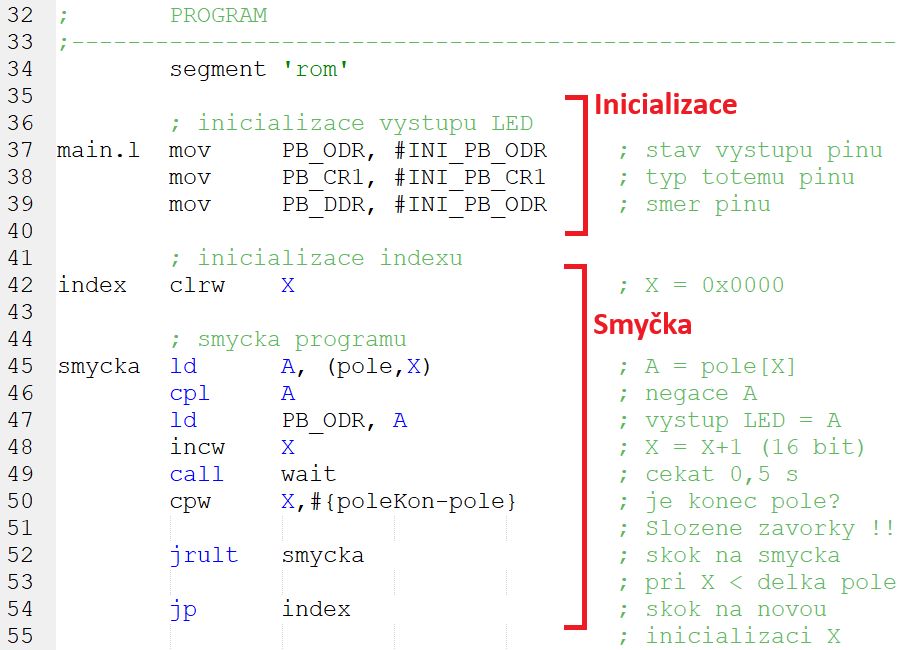
\includegraphics[width=0.80\textwidth]{fig/prg_pole_smycka.png}
		\end{center}
		
	\end{frame}
	
% =====================================================================================================================
	\begin{frame}
    \frametitle{Program - definice tabulky}
		
		\begin{center}
			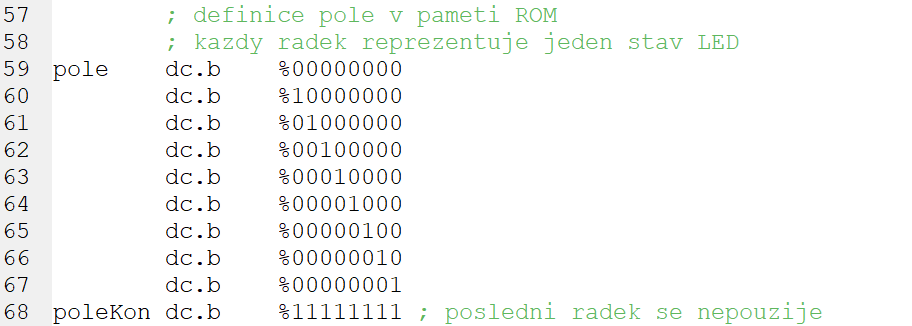
\includegraphics[width=0.80\textwidth]{fig/prg_pole_pole.png}
		\end{center}
		
		\begin{itemize}
			\item pole je definováno v segmentu \textbf{rom},
			\item direktiva \textcolor{blue}{\textbf{dc.b}} přímo zapisuje hodnotu do paměti,
			\item návěstí na konci je jen z důvodu snazšího určení délky tabulky (viz předchozí slide).
		\end{itemize}
		
	\end{frame}